\section{Introduction}

\begin{figure*}[h]
    \centering
    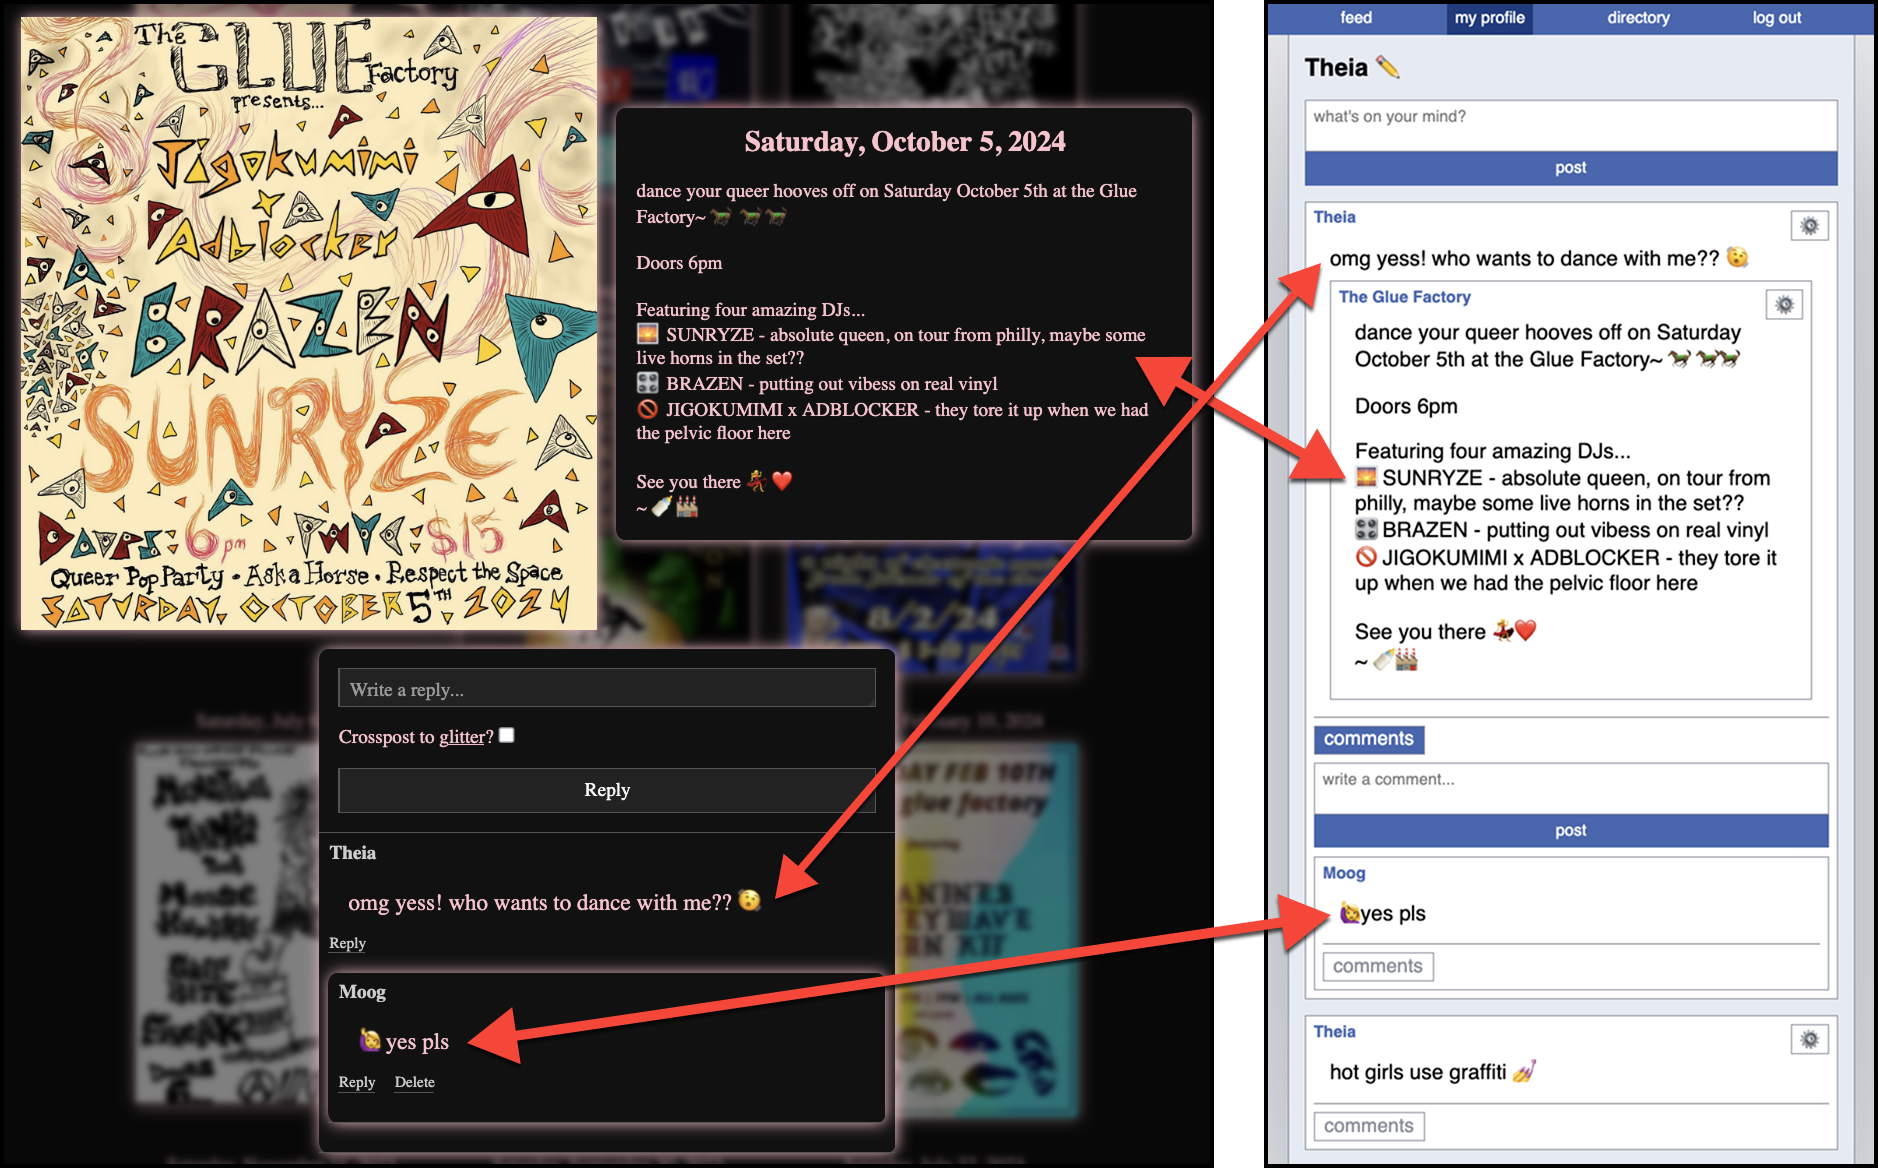
\includegraphics[width=\textwidth]{paper/figures/gloof-and-glitter.jpg}
    \caption{
    Interoperation between two applications built with Graffiti:
    The Glue Factory, an application operated by a venue to advertise their shows,
    and Glitter, a microblogging site.
    The show flyer visible in The Glue Factory is used with permission by the artist, Megan Levin.
    }
    \label{case-studies:fig:gloof-and-glitter}
\end{figure*}

Most social applications today are built like international airports,
designed to serve everyone, and soulless as a result.
Where are the online spaces that feel like
the unofficial skate park behind the grocery store,
the dance floor of a long-running nightclub,
or that one friend's living room?
Where are those intentional community spaces that
are not meant for everyone,
but are \emph{everything} to the people
who collectively curate their aesthetic and social norms?

Their absence is partly because truly personalized social applications
%DK given the framing you are using here, I wonder if "social web sites" is better than "social applications" (or if you need to use both and explain why).   Your examples---the nightclib, the friend's living room (and also Gloof) feel like sites not apps.   Per my email, it may be useful or necessary to talk somewhere in the paper about the difference between sites (you go there to interact with a certain kind of contet pertinent to the site?) ad apps (you pull in content from all over to interact with?) and how with gradfiti there is't really a differece
are extremely difficult to build,
and partly because the great power of social media---its
ability to connect massive numbers of people---also
creates social pressure for everyone to use the same few applications.

We present a system called \emph{Graffiti} that makes
building \emph{personalized} social applications
%and social sites with distinctive personalizities
more accessible,
while maintaining the interconnectedness that is special to social media.
We lay the foundation for developers to create a diverse ecosystem
of social applications
%and sites
with only client-side code and with minimal friction
to introducing new features,
while also ensuring that these applications \emph{interoperate},
allowing people to freely migrate between them without
losing their friends or data.
The types of social applications that can be built on the same set of Graffiti primitives range from analogs of Twitter to Facebook to Messenger to Slack to Goodreads to Pinterest to Wikipedia,
with plenty of room for entirely new creations.
%including social ``sites'' with distinctive personalities.

\hl{%
Our goal of interoperability leads almost immediately
to the conclusion that a user's
social data---their posts, likes, friend lists, and so on---\emph{cannot}
be stored within any single application.
Instead, user data is stored on a collective infrastructure
that all applications can access (subject to access control)
and selectively present data from according to their individual designs.
}%

\hl{%
This application-infrastructure separation
is an interoperability mechanism similar to
those used by
ActivityPub~{\cite{activitypub}},
which underlies Mastodon,
and the AT Protocol~{\cite{bluesky}}, which underlies Bluesky.
However, these social protocols---primarily designed to support
Twitter-like networked interactions---are limited in the range of applications
and features they can support.
Some limitations stem from hardwired assumptions,
like per-``instance'' moderation in ActivityPub
or the public-only visibility of content in the AT Protocol.
Other capabilities are technically \emph{possible}
but require standing up custom servers or navigating
a slow and complex standardization process.
% to perform out-of-band interactions.
In contrast, Graffiti provides a simple yet minimally constraining
client-side \emph{application programming interface} (API)
upon which a much broader range of personalized applications can be built, all
without server code or bureaucracy.
}%

% To illustrate the ecosystem this enables,
% suppose a group of friends start out by using an Instagram-like application,
% but some get bored of the interface and so by using the copy-and-paste
% programming that used to be popular on MySpace~\cite{copypasteliteracy}
% they make a ``fork'' of the application.
% Not everyone switches, which is fine because posts show up in either,
% but those who do get sparkly animations, the ability to
% add a colored halo around posts (to reflect their aura that day),
% and the ability to mark pictures of friends that look extra cute---the pictured
% friend can add the photo to their Tinder-like profile with a click.

% a group of users start using a Discord like server
% but then, largely from copy-and-pasting bits of
% code from other sites, like MySpace, they make it personal
% with features like X and Y.
% Unfortunately, an argument splits the group up,
% rather than one group getting custody of the app,
% they can continue on with two seperate ``views''.
% One application becomes popular and the other stays
% between a small group of friends, continually adding
% new features.
%DK maybe a simpler story, where an artist posts a new video on her "youtube channel", and a fan who is following her sees that post in his "twitter feed" and forwards it over "whatsapp" to his friends who talk about it there for a while with the result that eventually one of the friends uses "whatsapp" to "reply to" the original video post and that "reply" shows up as a comment on the artist's video on "youtibe".   Focus on the dyamics of the content without too much backstory about the participants.

% To achieve our goals of maximum personalization and interoperability, the "communication core" of Graffiti is kept as minimal and generic as possible, responsible only for delivering content from users' applications that post to to users' applications that want to access it; it can almost be thought of as a social analogue of TCP/IP.   All \emph{interpretation} of the transported content is left to the pure-client applications that create and consume it.  The communication core is so minimal that it only delivers \emph{notifications} about user posts, while the actual content of the users' posts can be kept in whatever personal storage those users' wish to use, such as their dropbox directories.  This again maximizes user control.


A key challenge of Graffiti's design is to resolve
the \emph{tension} between personalization and interoperability.
Allowing applications to have different styling is
not a problem, but can an application with top-down
moderation interoperate with a democratically moderated one?
Is it possible for a small community forum to exist and
not get flooded by the rest of the ecosystem's traffic?
We resolve these questions respectively with two concepts: \emph{total reification},
where all social interactions
are first-class objects that
can be interpreted or ignored by different applications;
and \emph{channels}, which organize data contextually,
preventing a phenomenon called ``context collapse''~\cite{contextcollapse}.


Our design decisions are guided by a set of \emph{requirements}, outlined
in Section~\ref{requirements}, that primarily focus on the direct experience
of social application developers and the users of their applications,
both users of Graffiti as a whole.
\hl{%
We include one additional requirement that targets the indirect
effects that \emph{power} over the underlying infrastructure
can have on the user experience.
Specifically, we leave room for users to retain control over their data
via technologies like decentralization or encryption.
}%

\hl{%
Importantly, however, Graffiti is not shaped by a particular
means of achieving this distribution of power. This again contrasts Graffiti
with systems like ActivityPub and the AT Protocol,
which are inseparable from their decentralized architectures
and leak architectural details, like ``instances'' and ``relays,''
into their APIs.
Graffiti's API-first\footnote{
We reply to the provocation ``\emph{Protocols, Not Platforms}''~{\cite{protocolsnotplatforms}},
the rallying cry that sparked Bluesky~{\cite{bluesky_from_protocols}},
with the amendment, ``\emph{...but the API first!}''
} approach not only reduces complexity for
developers who simply want to make applications,
but also allows the infrastructure underneath
to update as both technologies and threats evolve.
In fact, the Graffiti API is designed so that multiple implementations can exist
\emph{in parallel} underneath it,
allowing for the incremental adoption of new technologies,
similar to the web's transition from HTTP to HTTPS.
}%

After our requirements, we describe the Graffiti API,
first through high level concepts in Section~\ref{concepts},
then in detail in Section~\ref{api}.
Section~\ref{above-and-below} describes
the decentralized protocols we have built \emph{below} the API,
as well as the tooling we have developed \emph{above} the API
to build Graffiti applications with declarative and reactive programming.
In Section~\ref{case-studies},
we evaluate Graffiti through a series of case studies, demonstrating
how it is possible to build applications like Twitter, Messenger, and
Wikipedia, as well as novel applications on Graffiti, and how unusual
variants of all of these interoperate.
Finally, we wait until Section~\ref{related-work}
to continue exploring related work, by then with a more concrete
understanding of what we are relating to.
